\documentclass[../main.tex]{subfiles}
\usepackage[utf8]{inputenc}
\usepackage{blindtext}
\usepackage{float}
\usepackage{graphicx}
\usepackage{siunitx}

\begin{document}

In this section, we aim to address applications of Software Defined Satellites and how it's evolved over the years. Let's review what is meant by a software-defined satellite, Jeff Freedman, CEO of Kythera Space Solutions, defines a software-defined satellite as "having payloads that can be reconfigured using ground commands" \cite{podcast}. What allows for this reconfigurability is the inclusion of an on-board processor as well as a radio whose use can be modified. Some other components that could be defined via software are beamforming antennas, channeliszers, and demodulators/modulators (which we discussed were part of the SDR). \cite{podcast}

\section{Networks}
One of the increasing applications for Software-Defined Satellites has been in the domain of networks. Software-Defined Networking (SDN) have existed for some time now, since the release of the OpenFlow protocol SDNs have flourished \cite{sdn_architecture}.

Below shows a simplified view of an SDN architecture:

\begin{figure}[H]
    \centering
    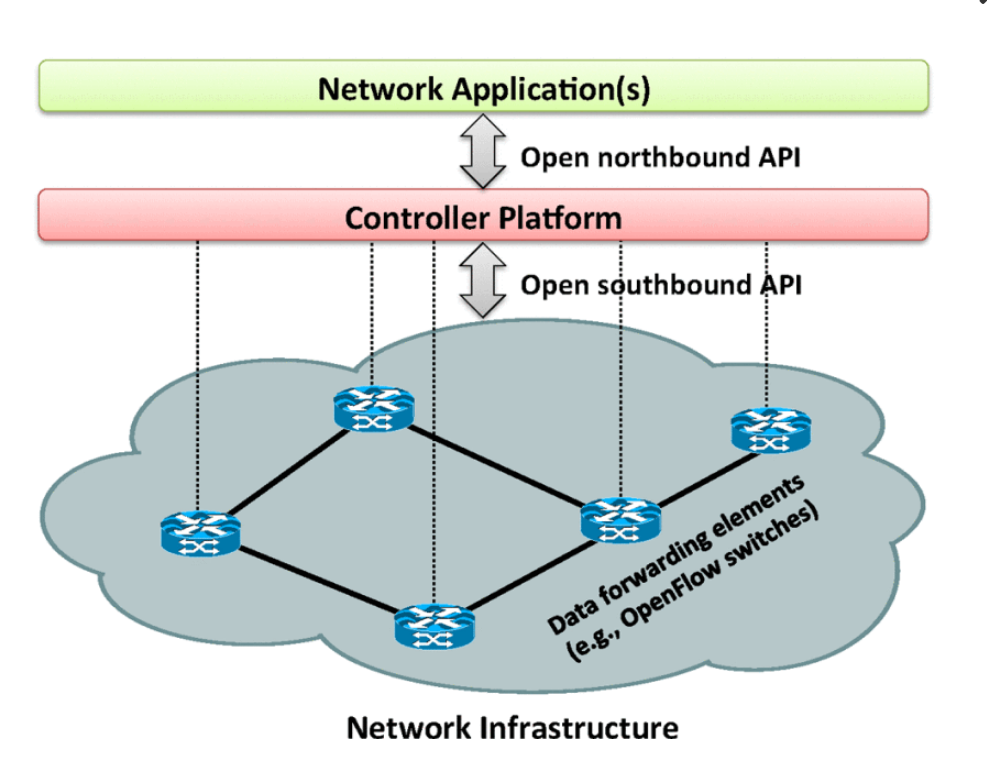
\includegraphics[width=300pt]{images/sdn_architecture.PNG}
    \caption{Simplified SDN Architecture}
    \label{fig:sdn}
\end{figure}

SDNs hope to change the limitations of current network infrastructure by breaking the vertical network integration into two components: the control plane and the data plane. The control plane is defined as the network's control logic, meaning it is responsible for calculating and installing the forwarding tables that exist on each and every router, as well as, determining how a datagram is routed among the routers along an end-to-end path from source to destination. The data plane, defined as the routers and switches that forward the traffic, in other words, the data plane is responsible for determining how a datagram arriving on an input port is forwarded to the router output port \cite{sdsn}. 

Tying this into software-defined satellite networks (SDSN), traditionally SDSNs depend on the closed and planned architecture, which makes configuration changes, the introduction of new communication and networking technologies, truly differentiated services provision, satellite network device interoperability, and the integration of satellite and terrestrial networks extremely difficult \cite{sdsn}.

As discussed above, SDNs provides flexibility, programmability, logical centralization, which increases network resource utilization, simplified network management, reduces operating cost, and promotes continuous improvement \cite{sdsn}.

\section{Flexibility}

Just the immense flexibility SDSs provide is a massive application. With SDSs you no longer need specific hardware for a specific mission, you can now use generic hardware to accomplish a myriad of missions. Satellite communications have always been very static and fixed but, SDSs provide dynamic beam coverage and ad-hoc configurability. One of the first SDSs launched was Eutelsat's Quantum satellite which features flexible architecture and customizable beam coverage. This satellite is able to adapt to commands regarding coverage, frequency bands, power use, and even it's orbital position. These are the benefits of a SDSs.

\end{document}